\documentclass{article}
\usepackage[utf8]{inputenc}
\usepackage{amsmath}
\usepackage{tabto}
\usepackage{graphicx}
\usepackage{tikz}
\usetikzlibrary{patterns}
\title{Exam 2}
\author{Intro to Robotics}
\date{Name: }

\begin{document}

\maketitle
\section{}
\textbf{1.} What is the equivalent quaternion to $R_{y'x'z'}(90^\circ, 180^\circ, 45^\circ)$ ?(foil has easiest arithmetic) \\\\
\textbf{2. }rotate the 3d vector $v_{1}=\begin{bmatrix}
0  \\
1 \\
0
\end{bmatrix}$ by the quaternion you obtained in part 1(use quaternion matrix multiplication for easiest arithmetic: formula 1). \newpage

\section{}
\begin{figure}[htp]
    \centering
    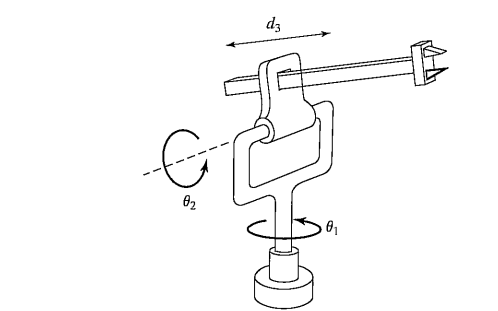
\includegraphics[width=10cm]{kinematics.png}
    \caption{Order of joints: revolute, revolute, prismatic(from bottom to top)}
    \label{fig:Arm}
\end{figure}\\
1. Draw the frames.\\
2. Compute DH table.\\\\
\begin{tabular}{ |p{3cm}|p{3cm}|p{3cm}| p{3cm} | p{3cm} |}
\hline
\multicolumn{5}{|c|}{DH table} \\
\hline
Frame \{i\} & \textbf{$a_{i-1}$} & \textbf{$\alpha_{i-1}$} & \textbf{$d_i$} & \textbf{$\theta_i$} \\
\hline
\textbf{1} &  &  &  &\\
\hline
\textbf{2} &  &  &  & \\
\hline
\textbf{3} &  &  &  & \\
\hline
\end{tabular}\\\\\\
3. Compute all transformation matrices.\\

\newpage

\section{}
Design a system using the publisher-subscriber model, for a robot that identifies boxes, picks them up, then takes them to a drop off location.
\newpage

\section{}
Assume you are given the functions move(speed, distance, is\_forward), rotate(angular\_speed, angle\_to\_rotate , is\_clockwise) :\\
1. Write a function that draws the letter H (make sure you draw nothing else on the grid, hint:you can retrace lines already drawn).\\


\newpage
\section{formulas}
\textbf{1. } $\begin{bmatrix}
a & -b & -c & -d\\
b & a & -d & c\\
c & d & a & -b \\
d & -c & b & a
\end{bmatrix}$\\\\
\textbf{2. } ${}^{i-1}_{i}T=\begin{bmatrix}
                c\theta_i & -s\theta_i & 0 & a_{i-1}\\
                s\theta_ic\alpha_{i-1} & c\theta_ic\alpha_{i-1} & -s\alpha_{i-1} & -s\alpha_{i-1}d_{i}\\
                s\theta_is\alpha_{i-1} & c\theta_is\alpha_{i-1}& c\alpha_{i-1} & c\alpha_{i-1}d_{i}\\
                0 & 0 & 0 & 1
               \end{bmatrix}$\\\\
\textbf{3.}$i^2=j^2=k^2=ijk=-1$ and \\\\
\begin{tabular}{ |p{3cm}|p{3cm}|p{3cm}| p{3cm} |}
\hline
\multicolumn{4}{|c|}{Multiplication Rules for Quaternions} \\
\hline
 & \textbf{i} & \textbf{j} & \textbf{k} \\
\hline
\textbf{i} & -1 & k & -j\\
\textbf{j} & -k & -1 & i\\
\textbf{k} & j & -i & -1\\
\hline
\end{tabular}\\
\end{document}
